%\textbf{The methodology was written before the finalised models and the mlpf inspired experimental model.  In order to make this methodology as comprehensive and readable as possible, we should consider to move out content to the appendix to free up space here. Consider what parts of the methodology that would be best to move to the appendix. The parts that are mostly practical and that does not have too much importance in chosen research  methodology related to the research question could be moved to the appendix.  ROOT reading could probably be moved to appendix.}

%\textbf{I should include a definition of permutation-invariant accuracy in methodology and I think that I should also include in this section as well the "can a global label swap recover the event?" plot that validates exactly this as an argument and then I should very clearly state that the accuracies that I report henceforth will be the permutation invariant accuracy, i.e the global swap permutation that yields the highest accuracy and then I should argue for why this accuracy is in fact the only interesting and relevant one for ldmx since electron has no inherent ordering and what we are in fact trying to achieve is electron shower separation and we are trying to form groups, there is no ordering difference the y-axis centroid ordering is a practical solution and just "arbitrarily" chosen}

% I want to communicate to the reader that much care and careful consideration went into these parts since I had the ambition that I would establish a platform that could be re-used and generalize for future deep learnig model implementations and optimizing models. Dont know where this is communicated best, maybe in start of methodology I think?

% Something in the style of "much care and effort went into implementing the root reading and tensorization, with the intention of establishing a platform, ml_ldmx, to allow for future studies and development of deep learning models on simulations of ldmx, either future student-projects or ldmx researchers. The intent is to implement a re-usable logic that extracts relevant information from ldmx simulations in root collections and pre-processes and prepares the data to apply deep learning models implemented in pytorch with these effectively and more easily. 

This chapter describes the complete experimental method: simulated event
production, construction of supervised targets and model-ready tensors, the
three neural-network architectures, their training procedures and the metrics
used for evaluation. 
% I like this formulation keep this or make it flow better with the text.
In simpler terms it could be said that this chapter will answer the question for the reader ''what was built, what was tested and how was it done?''. 

This chapter also presents and describes the intended reusable
\texttt{ml\_ldmx} framework \cite{ml_ldmx-github}, with the aim of separating
data conversion and target construction from any individual model. Simulation,
large-scale conversion and training were performed on the COSMOS Linux
\gls{hpc} cluster at Lund University with \gls{cpu} and \gls{gpu} resources available \cite{lunarc_cosmos}.

The chapter follows the processing chain from simulated events to supervised
targets, model inputs, neural-network training and evaluation. Technical
details that are more in-depth in nature necessary to reproduce this study
are collected in Appendix~\ref{sec:appendix}.


\subsection{Workflow and Reconstruction Tasks}


\subsubsection{Simulation and Data Pipeline Overview}
\label{sec:sim_overview}

Event production begins in the open-source \gls{ldmxsw} framework
\cite{ldmx-github}, which uses \gls{geant4} to simulate particle transport and
detector response \cite{geant4}. The physics single-electron \(1e\)
events are independently simulated and afterwards \textit{overlaid} to form \(2e\) and \(3e\) readout windows. Afterwards the detector response is simulated (''digitisation'') and
reconstruction algorithms are then performed on the combined detector deposits generating objects but also calculating energy readout. The
selected reconstructed quantities and simulation truth are extracted, within the \texttt{ml\_ldmx} framework, from the
resulting \texttt{ROOT} files and converted to variable-size \texttt{PyTorch}
tensors and stored in \gls{ml} model-ready \textit{''shards''}. Figure~\ref{fig:data_pipeline}
summarises this workflow from simulation to training in a high-level overview.

\begin{figure}[htbp]
    \centering
    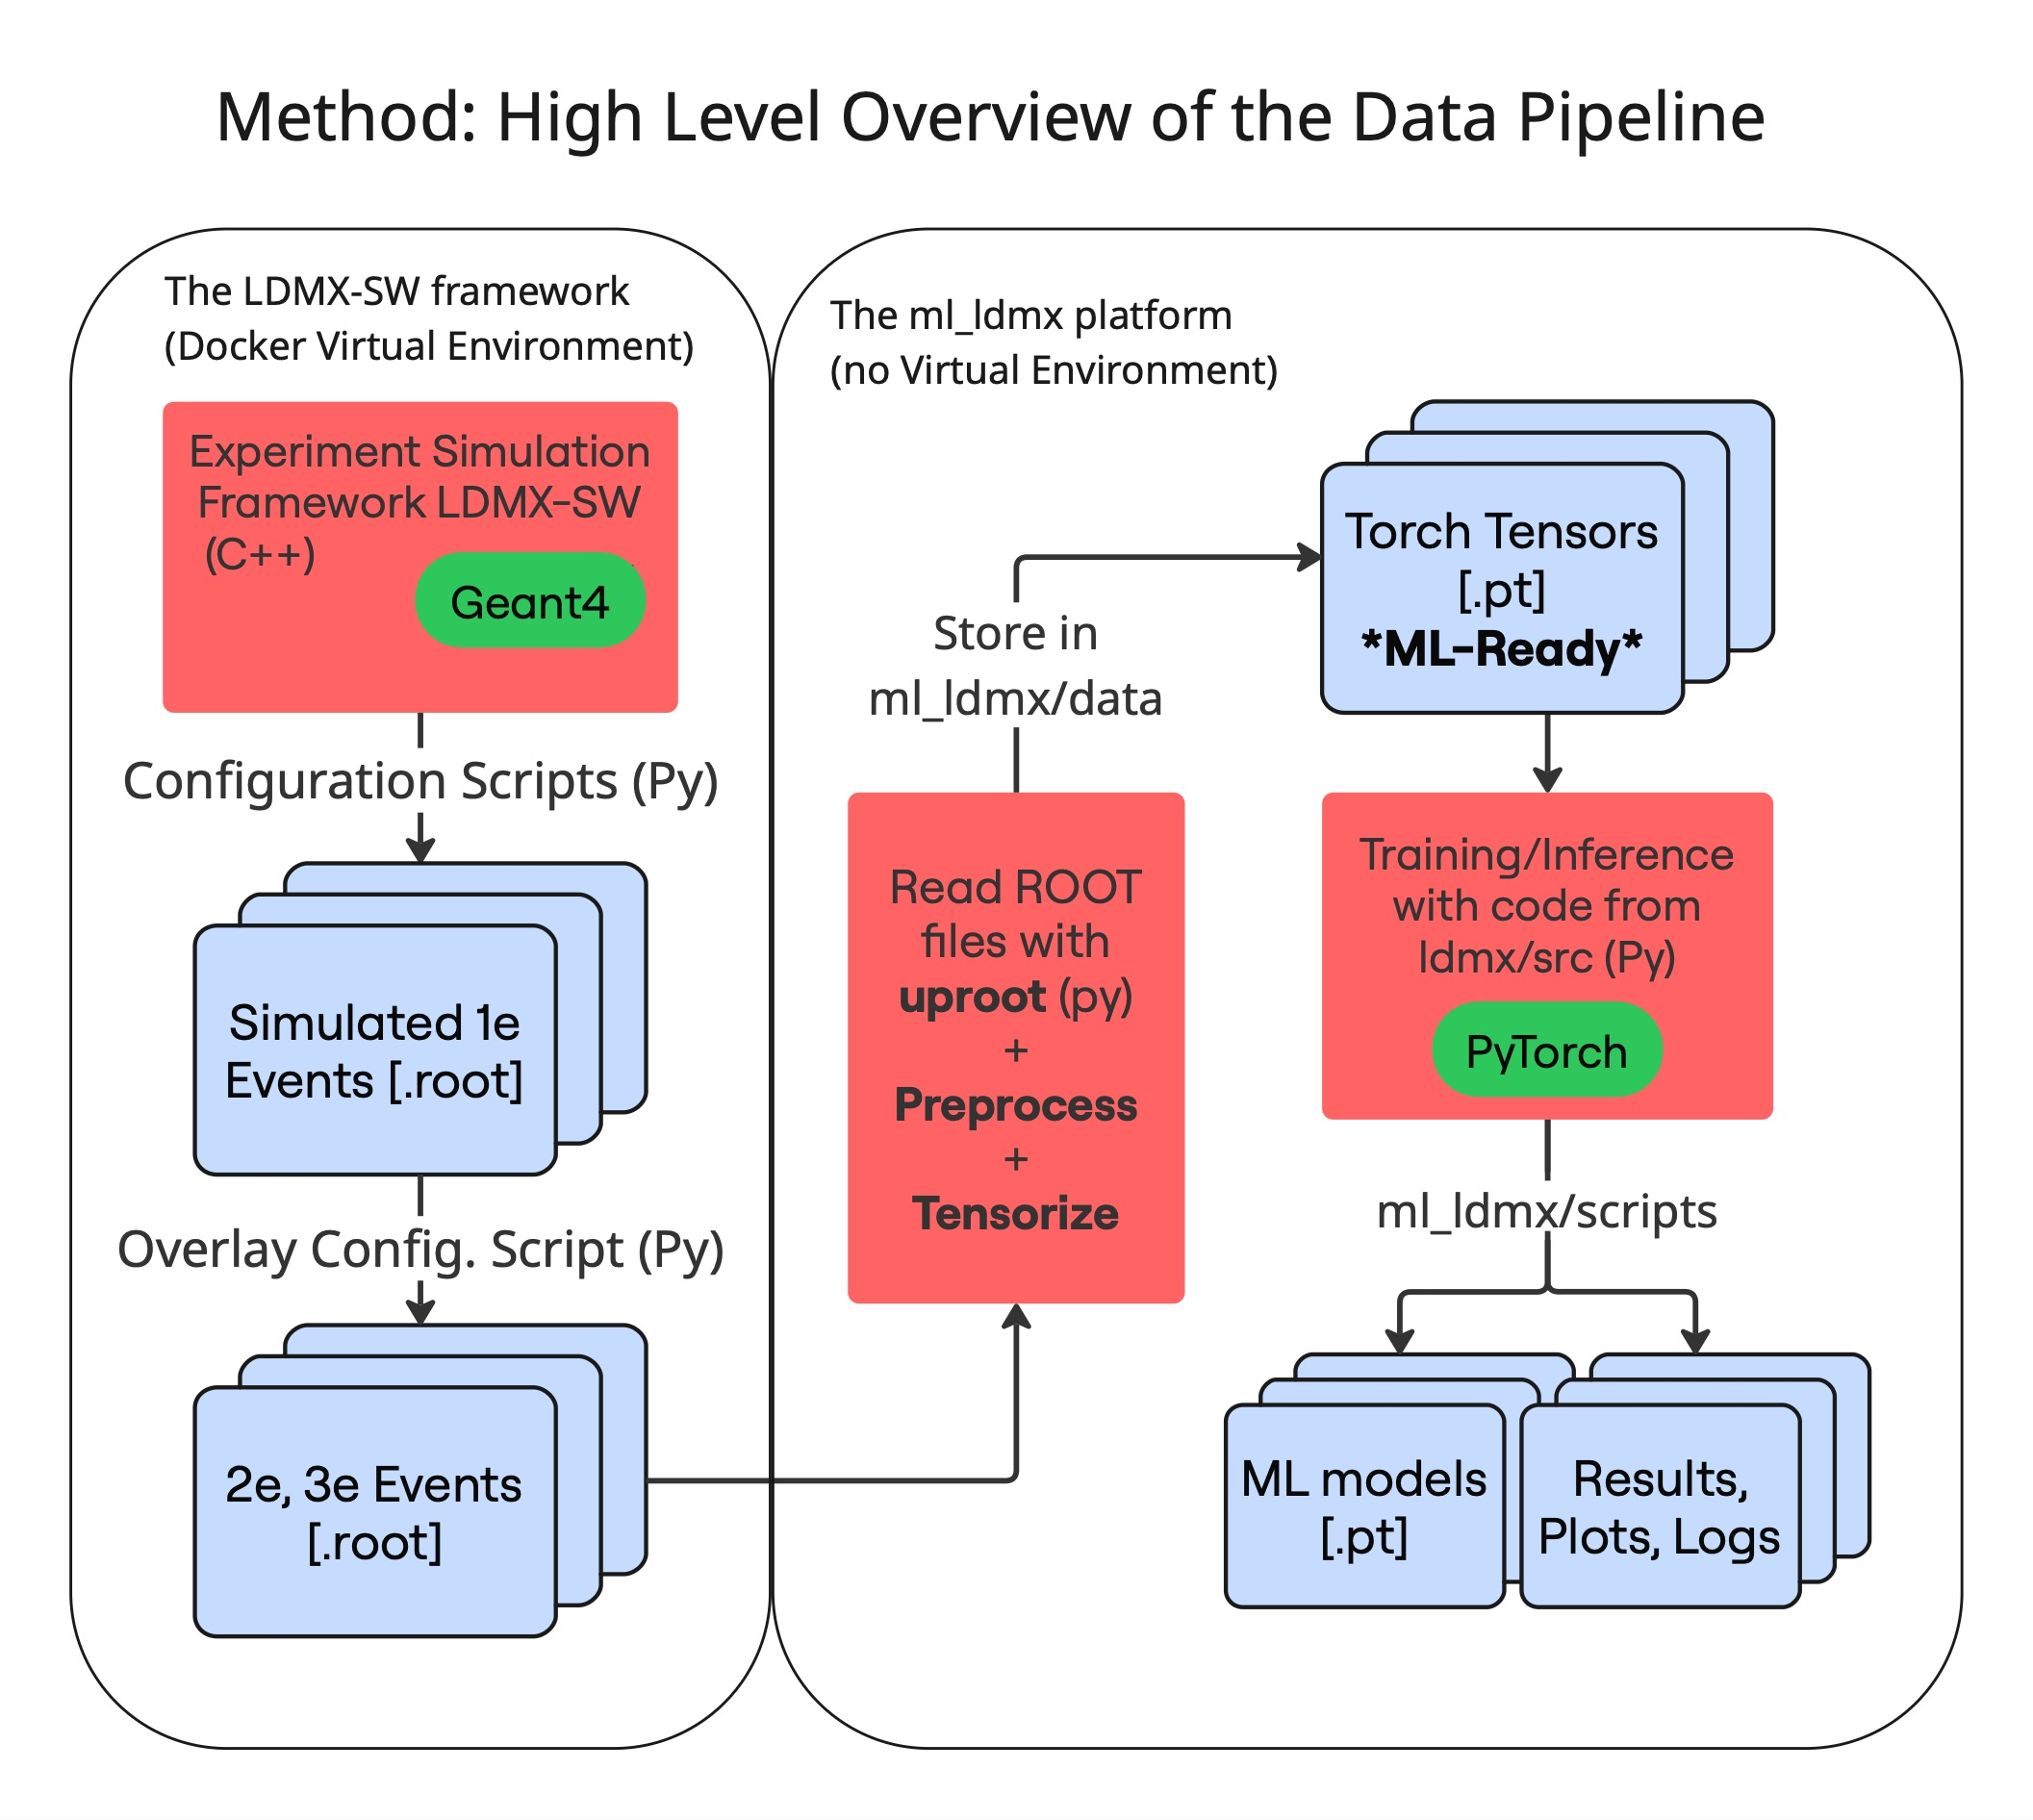
\includegraphics[width=0.85\textwidth]{config/fig/data_pipeline.jpg}
    \caption{High-level data flow pipeline from \gls{ldmx} simulation through target
    construction and tensorization to model training and evaluation.}
    \label{fig:data_pipeline}
\end{figure}



\subsubsection{Reconstruction Formulation}
\label{sec:reconstr_formulation}

For one event, the observed \gls{ecal} response is represented as the
variable-size set
\begin{equation}
    \mathcal{H} =
    \left\{
    \left(\boldsymbol{r}_i,E_i\right)
    \right\}_{i=1}^{N_{\mathrm{ECal}}},
    \qquad
    \boldsymbol{r}_i=(x_i,y_i,z_i),
\end{equation}
where $\mathcal{H}$ is the hit collection extracted from the \gls{ecal} subdetector, \(E_i\) is the reconstructed energy of hit \(i\) and $\boldsymbol{r}_i=(x_i,y_i,z_i)$ is the coordinates in 3D space. The standard event
representation also includes the variable-size set of
reconstructed \gls{ts} track observations
\begin{equation}
    \mathcal{T} =
    \left\{
    \left(c_j,n^{\mathrm{pe}}_j\right)
    \right\}_{j=1}^{N_{\mathrm{TS}}},
\end{equation}
where $\mathcal{T}$ is the collection extracted from the \gls{ts} subdetector, \(c_j\) is the reconstructed object of a one-dimensional track centroid and
\(n^{\mathrm{pe}}_j\) is the corresponding reconstructed number of
photoelectrons. The complete event input set is therefore represented by the pair
\(\mathcal{X}=(\mathcal{H},\mathcal{T})\), using an \gls{ecal}-only model view corresponds to the input set \(\mathcal{X}=\mathcal{H}\). 
% The \gls{ecal}-only model variants use the restricted input \(\mathcal{X}=\mathcal{H}\), omitting \(\mathcal{T}\).

%MATH HERE DEFINING TRIGGER SCINTILLATOR SET centroid and pe (variable size as well but low size nonetheless). It Previous paragraph should be rephrased as including ECal and TS data is standard and depending on the model the set omitts the set T from the TS. 

The principal supervised task is a \textit{node classification} task \cite{duarte2020-gnn-tracking} and each selected \gls{ecal} hit is assigned to the
electron contributing the largest simulated deposited energy in that cell.
As a simplified starting point, this fixed-multiplicity task is studied with GravNet and Transformer baselines.
Because a reconstruction method that is useful in practice should not require a known electron
count in advance, this motivated the more experimental \gls{trace} model, which
additionally predicts the valid electron slots in a mixed \(2e/3e\) sample,
the set of contributors and their energy fractions, drawing inspiration from
particle-flow reconstruction.

\subsection{Simulation}

The samples used in this study were produced with \gls{ldmxsw}. Its
versioned Docker\footnote{A Docker container is a portable software environment that packages
an application together with the dependencies needed to run it reproducibly
across different systems \cite{docker_container}.} container release captures the framework and its software
dependencies, including \gls{geant4}. The relevant configuration is summarized
in Table~\ref{tab:version_summary}; the exact simulation, overlay and
job-launch scripts are archived with the thesis code
\cite{ml_ldmx-github}. 

% TODO before submission: cite an immutable release or commit of the thesis repository.
\begin{table}[htbp]
    \centering
    \small
    \caption{Software and execution configuration used for event production.}
    \label{tab:version_summary}
    \begin{tabular}{p{0.27\linewidth} p{0.63\linewidth}}
        \hline
        Item & Configuration \\
        \hline
        Simulation framework & \gls{ldmxsw} container
        \path{ldmx/pro:v4.7.3} \\
        Detector geometry & \path{ldmx-det-v15-8gev} with the minimal
        scoring planes enabled \\
        Beam configuration & One \(8\,\mathrm{GeV}\) electron generated
        upstream of the tagging tracker \\
        Execution environment & \texttt{COSMOS} Linux \gls{hpc} cluster;
        jobs submitted with Slurm \\
        \hline
    \end{tabular}
\end{table}


\subsubsection{Single Electron ($1e$) Event Simulations}
\label{sec:1e_sim}

% the config script that generated the (altough maybe not exact) is found in
%/Users/eliotmontesinopetren/src/mpetren-msceng-ldmx/thesis_report/config_that_generated_single_electron_dataset.py

The single-electron source sample was generated with the configuration in
Table~\ref{tab:version_summary}, using the
\path{single_8gev_e_upstream_tagger()} beam generator. No interaction biasing
or event-level filter was applied.

The resulting events are referred to as \emph{inclusive}: they were not
selected for a particular interaction process. Instead, an electron was
delivered from the upstream beam position and its subsequent
interactions were determined by the transport simulation. The sample is
therefore dominated by electrons without a hard target interaction, while
\gls{sm} interactions remain present at their simulated rates
\cite{ldmx2025-overview}. No dark-sector signal process was injected. For clarity in this
report, the electrons drawn from this inclusive sample are called
\emph{non-signal electrons}. In the broader LDMX context they may also be
called \emph{pile-up electrons} when used as additional ''uninteresting'' interactions in an overlay. An existing source pool of about \(10^9\) such events was available for this study. 
%TODO: should I reference or credit Hans Alin in some way here? 
%Source files were assigned so that no simulated electron was reused in the generated multi-electron sample, a principle of \textit{unique} simulated electrons in every input event were held. The production logic details is found in Appendix~\ref{sec:appendix_overlay}.

\subsubsection{Multi-Electron (\(2e\) and \(3e\)) Event Simulation}
\label{sec:2e_sim}

Multi-electron, or \emph{pile-up}, events were constructed by overlaying
independently simulated single-electron interactions. The \gls{ldmxsw}
overlay combines their simulated physics and hit contributions by detector channel before the digitisation and reconstruction. The particles are transported independently (since $Z^{(k)} \perp\!\!\!\perp Z^{(\ell)}$),
but simulated detector response and reconstruction are repeated after overlay because
overlapping detector deposits must be processed jointly.

The configuration was based on the \gls{ldmxsw} in-time pile-up validation
workflow \cite{ldmx-github-itpileup}. Poisson sampling (of electron multiplicity) was disabled: every
output contained one main electron and either one or two overlaid electrons. Disjoint input source files were assigned so that no simulated electron was reused in the generated multi-electron sample, a principle of \textit{unique} simulated electrons in every input event were held. The production logic details is found in Appendix~\ref{sec:appendix_overlay}.

Figure~\ref{fig:event_displays} provides an example view of this construction.
The \(1e\) event contains one electron shower, whereas the \(2e\) and
\(3e\) events contain several truth-labelled hit groups in the same readout 
Their spatial overlap is the hit-classification problem addressed in this
thesis.

\begin{figure}[htbp]
    \centering
    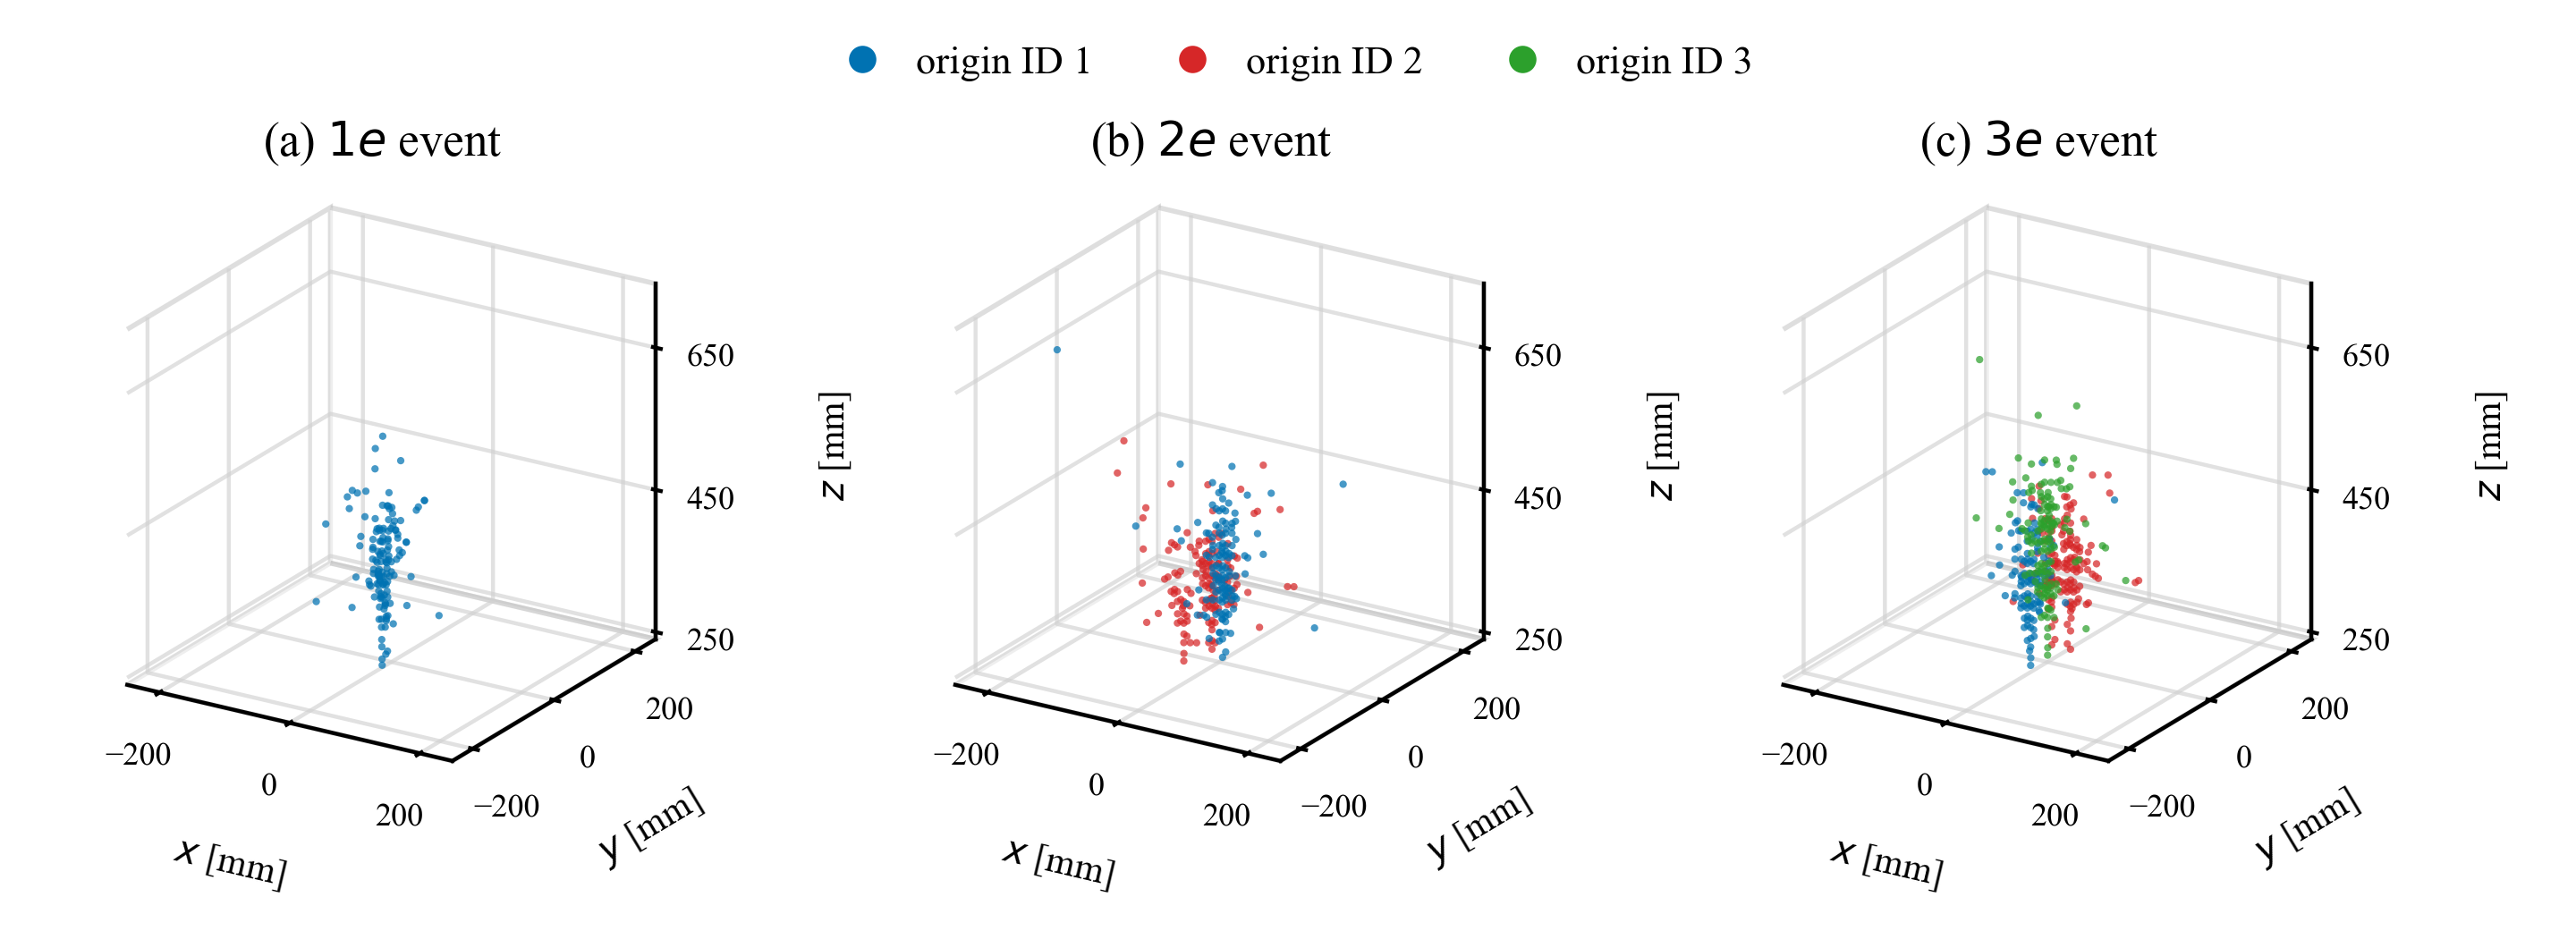
\includegraphics[width=\textwidth]{config/fig/ecal_truth_event_displays.png}
    \caption{Three-dimensional ECal event displays of randomly selected
    \(1e\), \(2e\) and \(3e\) events. Each marker represents a selected ECal
    hit and is coloured by the electron origin with the largest summed
    deposited-energy contribution to that hit. Noise hits are omitted and only
    simulation truth is shown; the event displays also represent a would-be perfectly predicted electron shower separation.}
    \label{fig:event_displays}
\end{figure}

The target of \(10^7\) events for each pile-up multiplicity was selected to
provide a large independent pool for model development and the study of
infrequent reconstruction failures. The resulting dataset contains
\(10^7\) events of each multiplicity. This sample size is not a direct test of the
experiment-level background rejection required by \gls{ldmx}: those
requirements are
process-specific and can reach twelve orders of magnitude for backgrounds
associated with few-\(\mathrm{GeV}\) bremsstrahlung
\cite{akesson2020-photon-veto}. 
The overlay release included an origin-identifier fix implemented by the
author so that source-electron labels remain available after overlay
\cite{petren2026-ldmx-origin-id-pr}. Table~\ref{tab:dataset_summary}
summarises the generated samples.

\begin{table}[htbp]
    \centering
    \small
    \caption{Sizes and construction of the inclusive (non-signal) event samples.}
    \label{tab:dataset_summary}
    \begin{tabular}{p{0.07\linewidth} p{0.27\linewidth}
                    p{0.14\linewidth} p{0.12\linewidth}
                    p{0.25\linewidth}}
        \hline
        Sample & Event construction & Events per file & Total events &
        Release \\
        \hline
        \(1e\) & Inclusive event \(8\,\mathrm{GeV}\) beam &
        \(10^4\) & \(\sim10^9\) & \texttt{ldmx-sw v4.6.2} \\
        \(2e\) & 1 main + 1 overlay electron &
        \(10^4\) & \(10^7\) & \texttt{ldmx-sw v4.7.3} \\
        \(3e\) & 1 main + 2 overlay electrons &
        \(5\times10^3\) & \(10^7\) & \texttt{ldmx-sw v4.7.3} \\
        \hline
    \end{tabular}
\end{table}


\subsection{Data Extraction and Supervised Targets}
\label{sec:method_processing}

This section defines the reconstructed detector quantities supplied to the
models and the simulation-only quantities used to construct targets. The
simulation and reconstruction output is stored in files with the
\texttt{.root} extension. ROOT is a C++ data-analysis framework widely used in
high-energy physics. Within each LDMX file, a \texttt{TTree} stores every
event as one entry and organises its quantities into compressed,
column-oriented branches. This provides space-efficient storage of the full
event record while allowing selected branches to be read efficiently
\cite{ROOT_NIMA_1997,root_about,root_ttree}.

\texttt{ROOT} reading, tensor and target construction, and model training are
deliberately kept as separate stages. This is a conscious design choice: the
\texttt{ROOT} files retain the broader simulation record, whereas conversion
extracts only the quantities required by this study into a reusable
model-ready representation. The conversion is therefore performed once rather
than repeated for every training run. Besides reducing repeated I/O and
preprocessing work, this keeps the target definition independent of the model
architecture and allows new models to use the same processed events.

Figure~\ref{fig:readout_vs_truth} shows the boundary between detector inputs
and simulation truth. Exact \texttt{ROOT} fields, reading logic and
intermediate data structures are given in
Appendix~\ref{sec:appendix_root_conversion}, together with the complete
conversion diagram in Figure~\ref{fig:io_and_tensor}.



\subsubsection{Selected Detector Data and Simulation Truth}

Only quantities available from reconstructed detector data are given to the
model. 
% Already introduced in reconstruction formulation %For an \gls{ecal} \gls{rechit}, these are the cell position and reconstructed energy, \((x_i,y_i,z_i,E_i)\). For a reconstructed \gls{tpad} track, they are the one-dimensional centroid and photoelectron count, \((c_j,n_j^{\mathrm{pe}})\).
The trigger-pad tracks provide context from another subdetector but do not
have their own hit-origin targets. Only \gls{ecal} hits have these targets.
The networks still produces a vector of class scores, called
\textit{logits}, for every input row. Before the loss and metrics are
calculated, the \texttt{ecal\_mask} selects only the ECal rows. Trigger-pad
rows can therefore influence the ECal predictions by context, but their own output
scores are ignored.

%TODO: THIS AND THE NEXT PARAGRAPH AND NEXT SUBSECTION HAS TO BE HARMONIZED. WE ARE TO USE THE RECHIT AND SIMHIT GLS
Detector-cell identifiers are used to match \gls{rechit} and
\gls{simhit} in the \gls{ecal} field. The deposited-energy and origin arrays describe
the energy in each stored contribution and the overlay origin to which it
belongs. Separate track identifiers describe the simulated tracks. The noise
flag is also used only when targets and dataset views are prepared. Truth is
therefore used to calculate the supervised loss and evaluation metrics, not
as a model input.

%TODO: THIS AND THE NEXT PARAGRAPH AND NEXT SUBSECTION HAS TO BE HARMONIZED. WE ARE TO USE THE RECHIT AND SIMHIT GLS
Simulation truth is used to construct targets and evaluation quantities, but
is never supplied as a model feature, as that would be cheating because these quantities 
are impossible to know in real life. Detector-cell identifiers match
reconstructed and simulated ECal hits, after which deposited-energy and origin
arrays determine the supervised targets. Trigger-pad tracks provide event
context but are not matched to the individual origin electron labels since that information 
was not implemented in the \gls{ldmxsw} simulations, thus not extractable. Event multiplicity
is retained as source metadata and, where required, as an evaluation target.
The exact input collections and fields are listed in
Table~\ref{tab:selected_root_fields} in
Appendix~\ref{sec:appendix_root_conversion}.


\begin{figure}[htbp]
    \centering
    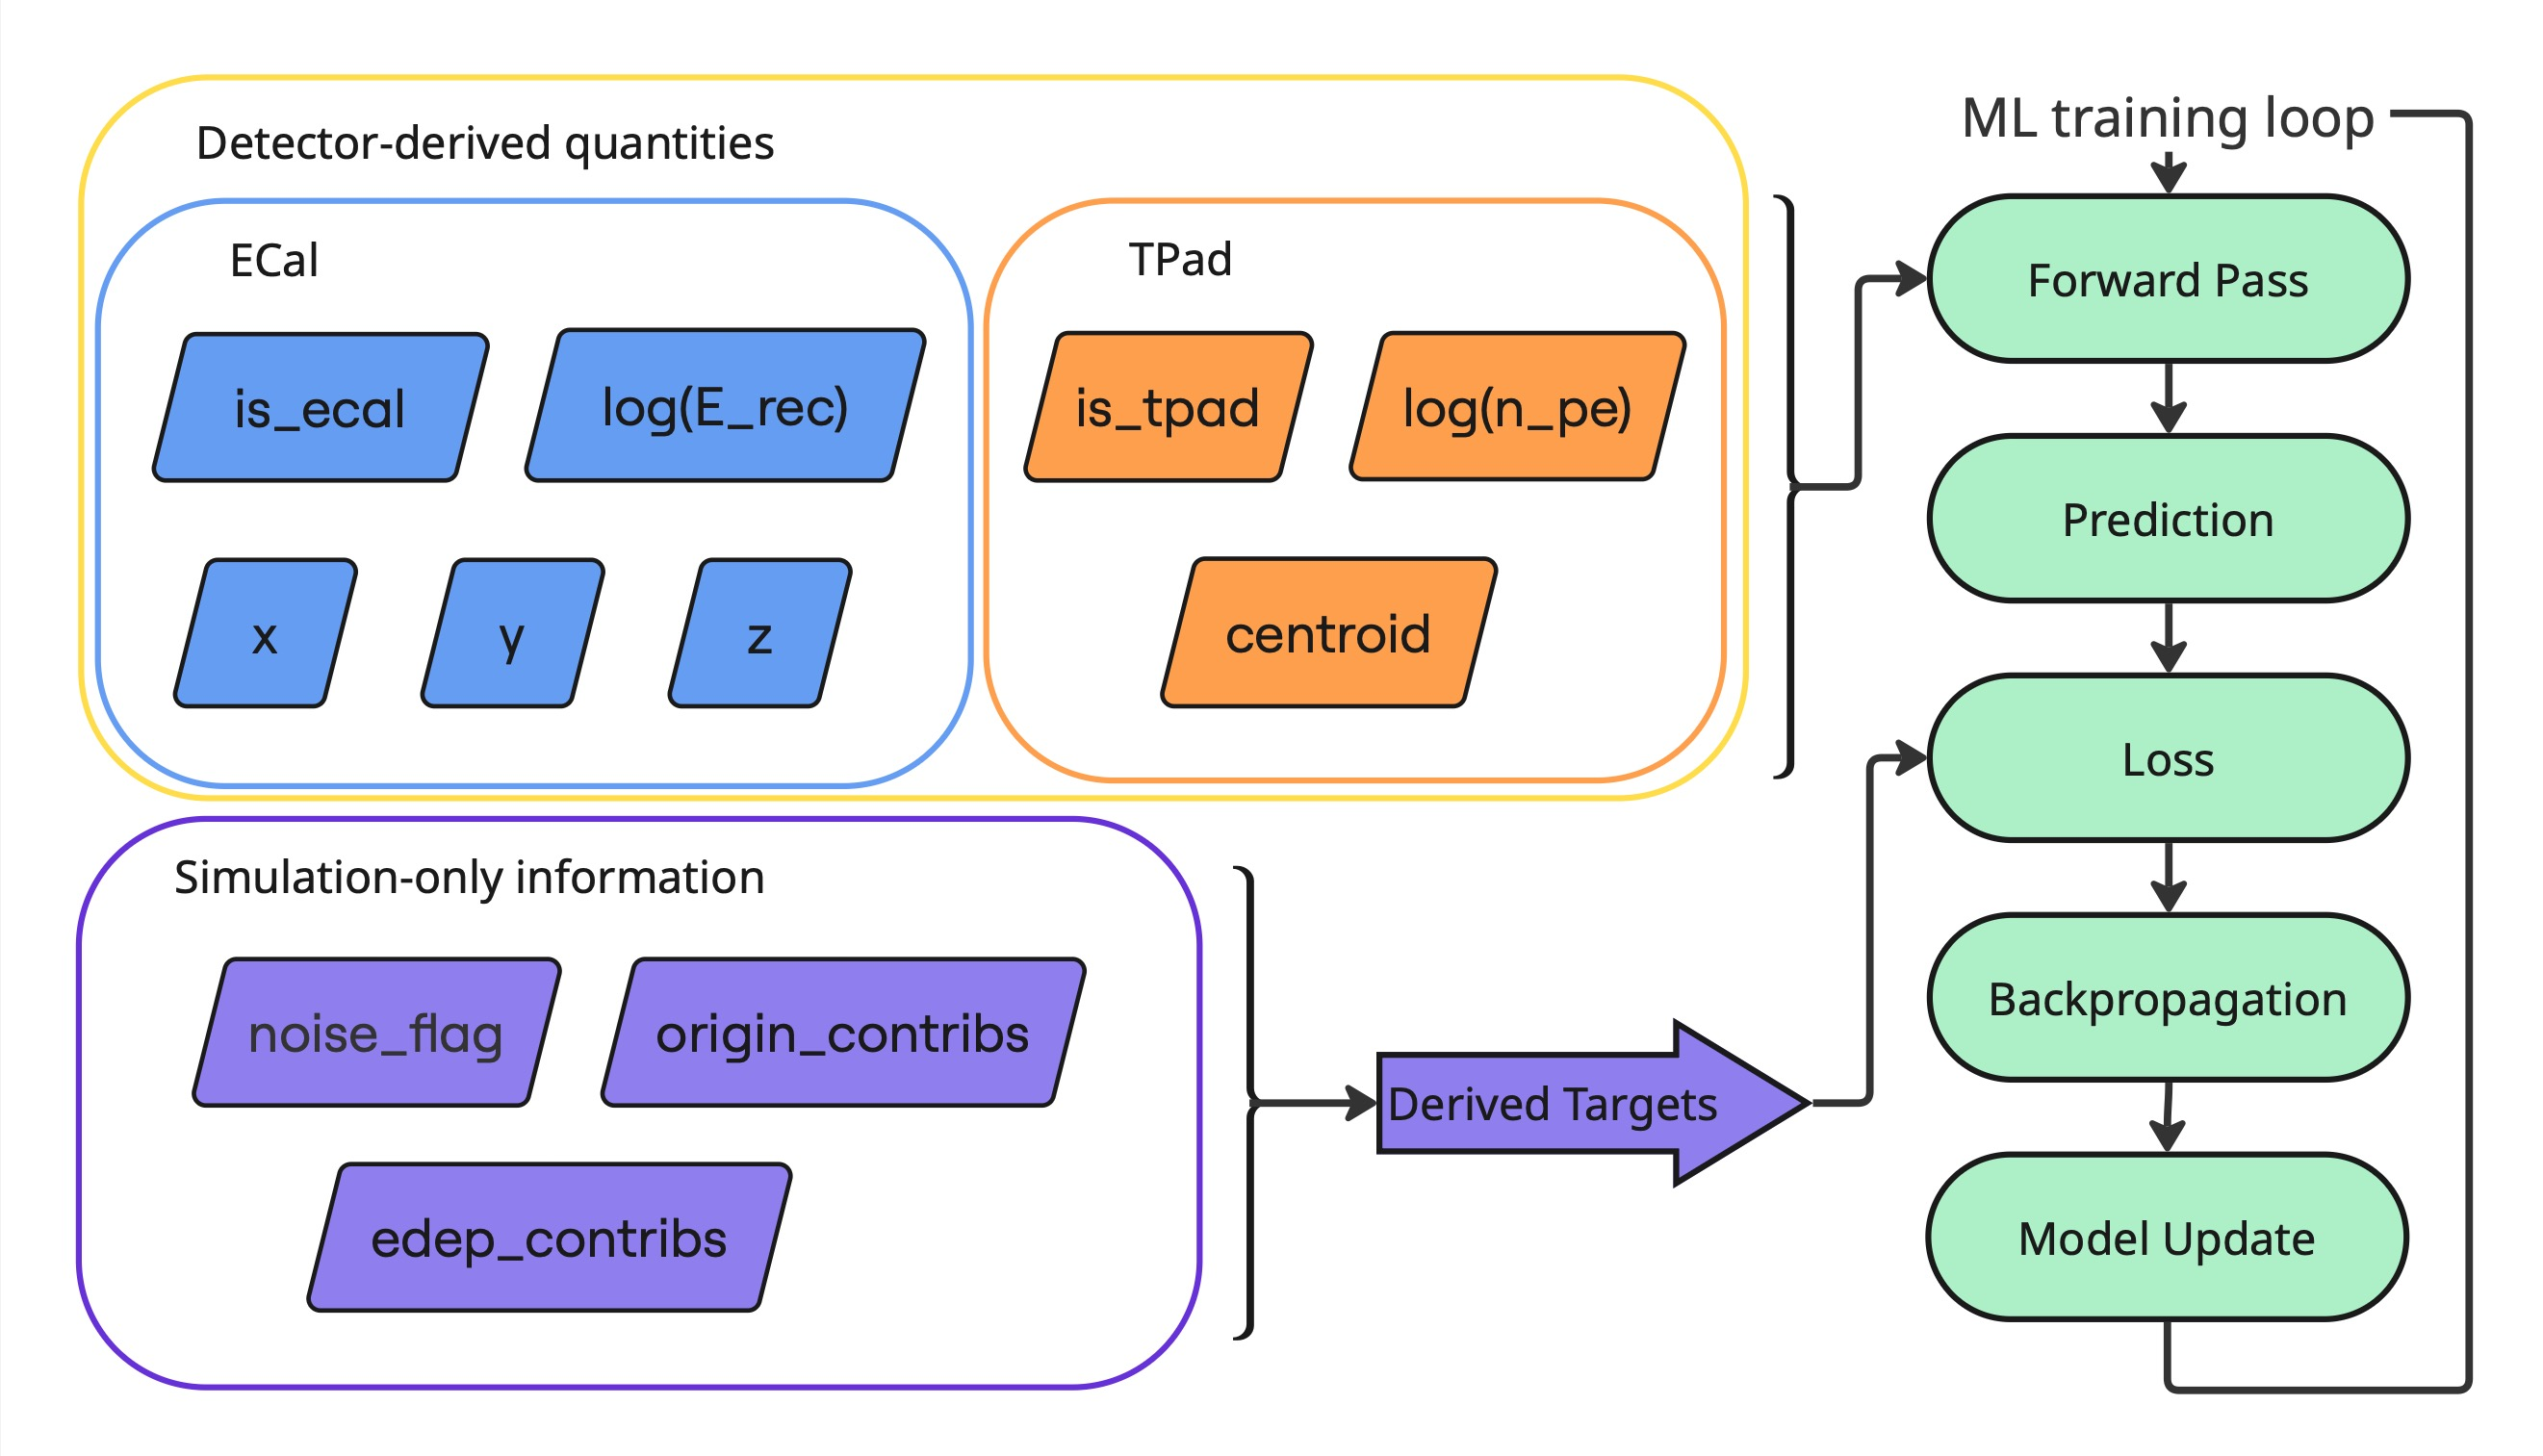
\includegraphics[width=\textwidth]{config/fig/readout_vs_truth.jpg}
    \caption{Use of detector-derived and simulation-only information in the
    supervised pipeline. Detector quantities form the model input, whereas
    simulation truth is used only to construct training targets and
    evaluation metrics.}
    \label{fig:readout_vs_truth}
\end{figure}


\subsubsection{Reconstructed-to-Simulated Hit Matching}

%TODO: THIS AND THE PREVIOUS PARAGRAPH AND PREVIOUS SUBSECTION HAS TO BE HARMONIZED. WE ARE TO USE THE RECHIT AND SIMHIT GLS
Reconstructed and simulated ECal collections can use different row orders.
They are therefore matched by detector-cell identifier while preserving the
reconstructed-hit order used by the model. A non-noise reconstructed hit must
have a corresponding simulated contribution in order to receive an origin
target; otherwise conversion stops rather than inventing a label. The
chunk-wise reading and intermediate record used for this operation are
described in Appendix~\ref{sec:appendix_root_conversion}.


\subsubsection{Target Definition and Baseline Simplifications}
\label{sec:method_targets}

The principal task assigns each selected ECal hit to the electron with the
largest deposited-energy contribution. To isolate this hit-assignment problem,
the baseline models make three simplifying assumptions:

\begin{enumerate}
    \item \textbf{Known electron count.} Each fixed-multiplicity baseline is
    trained and evaluated on either \(2e\) or \(3e\) events. The number of
    electron classes is therefore indirectly known before reconstruction and this isolates the hit-assignment task. A perhaps more desirable full-event reconstruction model (especially for online reconstruction) would also be assigned the task of predicting the number of electrons present. This lead to the experimental mixed-multiplicity model that relaxes this assumption and also infers the count.

    \item \textbf{One hard label per hit.} An \gls{ecal} cell may contain
    energy from several overlaid showers. For the baseline loss, the hit is
    assigned to only one origin label in \(\{1,2,3\}\), called the
    \textit{dominant origin}. It is the origin with the largest total
    deposited energy after contributions from the same origin have been summed.

    \item \textbf{Noise-free baseline input.} Simulated noise hits are kept in
    the reusable production shards but removed before data are given to a
    baseline model. The experimental model can instead retain them through a
    separate background class \(0\).
\end{enumerate}


\subsubsection{Dominant-Origin and Energy-Fraction Targets}

One reconstructed hit can contain several simulated energy contributions,
including multiple contributions from the same electron. Contributions with
the same overlay origin are therefore added first. Let \(D_{ij}\) denote the
total simulated energy deposited in hit \(i\) by electron \(j\).

The dominant-origin target is simply the electron that contributed the most
energy:
\begin{equation}
    y_i^{\mathrm{origin}}
    = \text{electron \(j\) with the largest \(D_{ij}\)}.
    \label{eq:dominant_origin_target}
\end{equation}
This single class label is used by the baseline classifiers and by the
dominant-origin evaluation of \gls{trace}.

The energy-fraction target retains the information discarded by the hard
label. For electron \(j\), it is
\begin{equation}
    f_{ij}
    =
    \frac{D_{ij}}{D_i^{\mathrm{total}}},
    \label{eq:origin_fraction_target}
\end{equation}
where \(D_i^{\mathrm{total}}\) is the total simulated energy deposited in the
hit. The fractions sum to one when the configured origins account for all of
that energy. The contributor-set target contains every electron with a stored
contribution to the hit. Thus, a hit can have one dominant-origin label while
still being represented as shared by several electrons.

An earlier implementation selected the origin associated with the largest
individual simulated contribution rather than first combining contributions
from the same electron. The summed rule was adopted because the target should
depend on the total energy from each physical origin, as that has a more meaningful physical interpretation. This correction produced
no measurable change in the reported model performance however.

\subsubsection{Noise Handling and Electron Ordering}

The production shards keep \gls{rechit}s that carry the simulation noise flag
and mark them with a Boolean noise target. Here, ``noise'' denotes a category
defined by simulation truth, not an estimate of unmodelled noise in detector
data. A noise hit is assigned to background class \(0\), and all of its
electron fractions are set to zero. Noise hits are removed before data are
given to a baseline model, whereas \gls{trace} can retain them as background.
Retained noise hits remain part of the event context, but they are excluded
when the set and ordering of electron origins are constructed.

The origin identifiers created during overlay merely distinguish the source
electrons; their numerical values have no consistent physical meaning between
events. Without a common convention, the same output class could refer to the
upper shower in one event and the lower shower in another. The electrons are
therefore assigned canonical labels using their transverse \(y\)-positions.

For each electron, the ordinary, unweighted mean \(y\)-coordinate is calculated
from the non-noise ECal hits for which that electron is the dominant origin.
The electrons are then sorted from the lowest to the highest mean
\(y\)-coordinate and assigned consecutive classes: the lowest becomes class
1, the next class 2, and, in a \(3e\) event, the highest class 3. The
energy-fraction columns are reordered in the same way.

This changes the class labels only. It does not sort the tensor rows, weight
positions by energy, use trigger-pad centroids or match trigger-pad tracks to
electron origins. The saved shards contain the original physical-origin
labels. Canonical-\(y\) labels are constructed when the data are loaded. The
original origin identifiers and fraction-column order are kept so the mapping
can be traced.

\subsection{Tensorization and Model-Ready Data}
\label{sec:method_features}

% First we should say what tensorization is, which is kind of said now. 
Each temporary event record is converted into numerical arrays, masks, targets and metadata suitable for model training. Events keep their variable size and the stored order within each detector collection. 

\subsubsection{Combined Event Tensor}

Let \(N_{\mathrm{E}}\) and \(N_{\mathrm{T}}\) be the total number of retained
\gls{ecal} hits and trigger-pad tracks in an event respectively. The \gls{ecal} rows are placed
first and the trigger-pad rows follow:
\begin{equation}
    \mathbf{X}
    \in
    \mathbb{R}^{(N_{\mathrm{E}}+N_{\mathrm{T}})\times 8},
    \qquad
    \mathbf{x}_n =
    \begin{cases}
        (1,0,x_i,y_i,z_i,\widetilde{E}_i,0,0),
        & n=i, \\[2mm]
        (0,1,0,0,0,0,c_j,\widetilde{n}^{\mathrm{pe}}_j),
        & n=N_{\mathrm{E}}+j .
    \end{cases}
    \label{eq:combined_event_tensor}
\end{equation}
% This could be shown visually in a very nice way but that improvement comes at a later stage (if there is still time left before the deadline!) so in flowing text is fine for now.
The first two columns are the row-type flags \texttt{is\_ecal} and
\texttt{is\_tpad}. Columns 3--6 contain \texttt{ecal\_x},
\texttt{ecal\_y}, \texttt{ecal\_z} and \texttt{ecal\_energy}; the final two
contain \texttt{tpad\_centroid} and \texttt{tpad\_pe}. Fields that do not
apply to a row are filled with zeros. The type columns and corresponding
\texttt{ecal\_mask} and \texttt{tpad\_mask} identify the row type. Hit-level
targets and losses apply only to the \(N_{\mathrm{E}}\) ECal rows, while
trigger-pad rows provide context.

An \gls{ecal}-only model view selects
\((x_i,y_i,z_i,\widetilde{E}_i)\) from the same stored event rather than
using a second processed dataset, so the combined event tensor can be utilized by all trained models. The collection order is preserved in
storage, but the row index has no physical meaning for the models. \gls{ecal} hits
and \gls{tpad} tracks are treated as unordered sets with variable size.

\subsubsection{Preprocessing of Energy Input Features}
\label{sec:preprocess}

The production shards used in this study apply a log transform of the energy-based features that are present in the input
\begin{equation}
    \widetilde{E}
    = \log\!\left(1+\max(E,0)\right),
    \qquad
    \widetilde{n}^{\mathrm{pe}}
    = \log\!\left(1+\max(n^{\mathrm{pe}},0)\right),
    \label{eq:input_log_transforms}
\end{equation}
using the \texttt{log1p} function in \texttt{PyTorch}
\cite{pytorch_log1p}. Both input distributions are right-skewed, as is typical
for intensity-valued energy features \cite{lai2024shower}. These
transforms reduce their numerical range while preserving the order of the
values, making them numerically more suitable for \gls{ml}. Deposited energies
used only to construct truth targets remain on their original scale. The input
distributions before and after transformation are shown in
Figure~\ref{fig:skew_and_log} in
Appendix~\ref{sec:appendix_tensor_storage}.

\subsubsection{Model-Ready Dataset}

Converted events are stored in versioned \texttt{PyTorch} shards containing
the model inputs, detector masks, targets, raw values needed for evaluation
and source metadata. Unlike the complete \texttt{ROOT} event record, these
shards are a task-specific training representation and do not duplicate
unused simulation content. Training can therefore read the converted tensors
directly without reopening the source files or reconstructing targets, while
the retained metadata preserves traceability to the source event. The stored
schema, provenance manifests, indexing and caching strategy are documented in
Appendix~\ref{sec:appendix_tensor_storage}.


\subsubsection{Data Split and Training-Time Preparations}


% the test split can be presented in a small "wrap-table" that is on the right hand side of the text that would be nice. 
The event indices are shuffled with a fixed seed and divided into training,
validation and test sets. The proportions are \(80\%\), \(10\%\) and \(10\%\) respectively.
Only the index lists are split, so the shards do not need to be rewritten.
For a baseline model, noise rows are removed and the physical-origin labels
are mapped to canonical-\(y\) classes when each event is loaded.

% "Continous columns" was difficult to understand not intuitive for the reader and I added text that are necessary to explain better it has to be referenced with the entries that are integers or float values, but there is a better way to explain this that flows better... something more intuitive had to be added that references to the equation 
%How are they standardized? What does that mean specifically? Are they normalized into a range like from 0 to 1? IS THE LOG TRANSFORM PREPROCESSING BEFORE OR AFTER THIS?
After the split, the six continuous columns 3--6 in
Equation~\eqref{eq:combined_event_tensor} are standardized using means and
standard deviations calculated from the training set only. The two binary
detector-type columns are not standardized. The same training statistics are
applied to validation and test data and saved with the model run. Scaling is
fitted on the common heterogeneous representation before a model-specific
view is selected; implementation details are given in
Appendix~\ref{sec:appendix_tensor_storage}.











\subsection{Model Architectures}
\label{sec:method_models}


\subsubsection{Capacity-Selection Strategy}
\label{sec:method_capacity_selection}

Model capacity was selected with a performance-first strategy. The principal
objective was to establish whether the proposed inputs and interaction
mechanisms could achieve useful reconstruction performance, rather than to
identify the smallest possible network. Widths and depths were therefore
chosen conservatively from development runs so that insufficient capacity was
unlikely to be the dominant limitation. The scale of contemporary
Transformer-based \gls{mlpf} implementations provided a qualitative reference
for a reconstruction model with heterogeneous inputs
\cite{pata2026-mlpf}. The present LDMX task nevertheless has \emph{much} smaller input
sets and also a narrower output scope than full CMS particle-flow reconstruction.

This study did not either include a broad hyperparameter or architecture sweep, nor
did it attempt pruning, quantisation, knowledge distillation or another model
compression procedure. Thus, the reported parameter counts should not be interpreted as
minimum capacities required by the reconstruction tasks. Establishing the
accuracy--latency--memory trade-off is left to future work.

The architectures reported below are the configurations used for the
million-event training campaigns found in the results. Separate \(2e\) and \(3e\) models were
trained within each baseline family, but their architectures and
hyperparameters are identical except for the width of the final classifier:
\(C=2\) for the \(2e\) task and \(C=3\) for the \(3e\) task. Each baseline model used one million
fixed-multiplicity events, whereas the contributor-set slot model used one
million events balanced between the \(2e\) and \(3e\) sources not informing the model the multiplicity count beforehand.



\subsubsection{GravNet Baseline}

The GravNet baseline embeds every eight-feature ECal or trigger-pad node in a
128-dimensional latent space. Four residual \texttt{GravNetConv} blocks then
learn event-local neighbourhoods and propagate information between nearby
nodes in the learned space \cite{qasim2019-gravnet}. A linear per-node head
produces the origin logits, of which only the ECal rows are supervised. The
graph-assignment vector described in
Section~\ref{sec:method_batching} prevents message passing between events. The selected baseline architectures are summarised side by side in
Figure~\ref{fig:baseline_architectures}.

\subsubsection{Transformer Baseline}

The Transformer baseline maps the same eight input features to a
128-dimensional representation and applies three pre-layer-normalised
encoder blocks. Within each event, full self-attention lets every valid token
interact with every other valid token and the padding mask prevents padded rows
from contributing, and the leading batch dimension is processed
independently. A linear token head produces the ECal hit-origin logits. This
model adds no sequence positional encoding and the detector coordinates are already
included in the input features, and the row order carries no meaning. This
set-to-set construction follows the interaction pattern used in recent
\gls{mlpf} models while retaining and restricting it to a single \gls{ldmx}-specific output task
\cite{pata2026-mlpf}. The selected baseline architectures are summarised side by side in
Figure~\ref{fig:baseline_architectures}.

\begin{figure}[p]
    \centering
    \begin{minipage}[t]{0.48\textwidth}
        \centering
        \vspace{0pt}
        \textbf{(a) GravNet baseline}\par\vspace{3mm}
        \begin{tikzpicture}[
            >=Latex,
            node distance=5mm,
            every node/.style={font=\normalsize},
            stage/.style={draw, rounded corners, align=center,
                         minimum height=14mm, text width=62mm,
                         fill=RoyalBlue!8},
            block/.style={draw, rounded corners, align=center,
                         minimum height=28mm, text width=62mm,
                         fill=ForestGreen!11},
            arrow/.style={->, thick}
        ]
            \node[stage] (g-input) {
                \textbf{Mixed detector nodes}\\
                ECal and trigger-pad rows,\\
                \(\mathbf{X}_{\mathrm{cat}}
                \in\mathbb{R}^{N_{\Sigma}\times 8}\)
            };
            \node[stage, below=of g-input] (g-projection) {
                \textbf{Input projection}\\
                \(\operatorname{Linear}(8,128)\)\\
                \(\rightarrow\operatorname{ReLU}\)
            };
            \node[block, below=of g-projection] (g-gravnet) {
                \textbf{GravNet residual block}\\
                \(\boldsymbol{\times 4}\)\\
                \(\operatorname{GravNetConv}(128,128;\)\\
                \(d_s=4,\ d_p=128,\ k=16)\)\\
                \(\rightarrow\operatorname{ReLU}
                \rightarrow\operatorname{Dropout}(0.1)\)\\
                \(\rightarrow\text{residual addition}\)\\
                \(\rightarrow\operatorname{BatchNorm1d}(128)\)
            };
            \node[stage, below=of g-gravnet] (g-head) {
                \textbf{Per-node classification head}\\
                \(\operatorname{Linear}(128,C)\), with\\
                \(C=2\) for \(2e\) and \(C=3\) for \(3e\)
            };
            \node[stage, below=of g-head] (g-output) {
                \textbf{ECal-supervised output}\\
                Select ECal-node logits;\\
                trigger-pad nodes provide context only
            };

            \draw[arrow] (g-input) -- (g-projection);
            \draw[arrow] (g-projection) -- (g-gravnet);
            \draw[arrow] (g-gravnet) -- (g-head);
            \draw[arrow] (g-head) -- (g-output);
        \end{tikzpicture}
    \end{minipage}%
    \hfill
    \begin{minipage}[t]{0.48\textwidth}
        \centering
        \vspace{0pt}
        \textbf{(b) Transformer baseline}\par\vspace{3mm}
        \begin{tikzpicture}[
            >=Latex,
            node distance=5mm,
            every node/.style={font=\normalsize},
            stage/.style={draw, rounded corners, align=center,
                         minimum height=14mm, text width=62mm,
                         fill=RoyalBlue!8},
            block/.style={draw, rounded corners, align=center,
                         minimum height=38mm, text width=62mm,
                         fill=Orange!14},
            arrow/.style={->, thick}
        ]
            \node[stage] (t-input) {
                \textbf{Padded mixed-detector tokens}\\
                ECal and trigger-pad rows,\\
                \(\mathbf{X}_{\mathrm{pad}}\in
                \mathbb{R}^{B\times N_{\max}\times 8}\)
            };
            \node[stage, below=of t-input] (t-projection) {
                \textbf{Input projection}\\
                \(\operatorname{Linear}(8,128)\)\\
                \(\rightarrow\operatorname{ReLU}\)\\
                \(\rightarrow\operatorname{Linear}(128,128)\)
            };
            \node[block, below=of t-projection] (t-encoder) {
                \textbf{Pre-layer-normalised}\\
                \textbf{Transformer encoder block}\\
                \(\boldsymbol{\times 3}\)\\
                \(\operatorname{LayerNorm}(128)\)\\
                \(\rightarrow\text{four-head full self-attention}\)\\
                \(\rightarrow\operatorname{Dropout}(0.1)\)\\
                \(\rightarrow\text{residual addition}\)\\
                \(\operatorname{LayerNorm}(128)\)\\
                \(\rightarrow\text{FFN }128\!\rightarrow\!256
                \!\rightarrow\!128\)\\
                (ReLU, dropout \(0.1\))\\
                \(\rightarrow\text{residual addition}\)
            };
            \node[stage, below=of t-encoder] (t-finalnorm) {
                \textbf{Final encoder normalisation}\\
                \(\operatorname{LayerNorm}(128)\)
            };
            \node[stage, below=of t-finalnorm] (t-head) {
                \textbf{Per-token classification head}\\
                \(\operatorname{Linear}(128,C)\), with\\
                \(C=2\) for \(2e\) and \(C=3\) for \(3e\)
            };
            \node[stage, below=of t-head] (t-output) {
                \textbf{ECal-supervised output}\\
                Select ECal-token logits;\\
                trigger-pad tokens provide context only
            };

            \draw[arrow] (t-input) -- (t-projection);
            \draw[arrow] (t-projection) -- (t-encoder);
            \draw[arrow] (t-encoder) -- (t-finalnorm);
            \draw[arrow] (t-finalnorm) -- (t-head);
            \draw[arrow] (t-head) -- (t-output);
        \end{tikzpicture}
    \end{minipage}
    \caption{Architectures of the selected (a) GravNet and (b)
    pre-layer-normalised Transformer baselines. For GravNet, the learned-space
    dimension is \(d_s=4\), the propagated-feature dimension is \(d_p=128\),
    and each learned neighbourhood contains \(k=16\) nodes. The Transformer
    has model width 128, feed-forward width 256, and four attention heads of
    dimension 32.}
    \label{fig:baseline_architectures}
    \label{fig:gravnet_baseline_architecture}
    \label{fig:transformer_baseline_architecture}
\end{figure}



\subsubsection{TRACE: Multi-Task Contributor Reconstruction}

The proposed model uses one shared Transformer backbone for the mixed
\(2e/3e\) dataset. A learned detector-type embedding distinguishes ECal and
trigger-pad tokens. Two ECal-supervised heads predict the subset of electron
slots contributing to each hit and their energy fractions. In parallel, a
mask-aware event summary predicts which of the three electron slots are
valid. Coherent post-processing combines these outputs to derive the electron
count, dominant hit origin and pure-versus-mixed classification and these are
not learned by separate heads. The three training losses: contributor-set,
fraction and slot-validity, were assigned equal weight.

\begin{figure}[H]
    \centering
    \begin{tikzpicture}[
        >=Latex,
        node distance=4mm and 3mm,
        every node/.style={font=\normalsize},
        shared/.style={draw, rounded corners, align=center,
                      minimum height=12mm, text width=108mm,
                      fill=RoyalBlue!8},
        encoder/.style={draw, rounded corners, align=center,
                       minimum height=18mm, text width=108mm,
                       fill=Orange!14},
        token/.style={draw, rounded corners, align=center,
                     minimum height=29mm, text width=58mm,
                     fill=ForestGreen!11},
        event/.style={draw, rounded corners, align=center,
                     minimum height=29mm, text width=58mm,
                     fill=Purple!10},
        arrow/.style={->, thick}
    ]
        \node[shared] (embedding) {
            \textbf{Padded mixed-detector input and embedding}\\
            \(\mathbf{X}_{\mathrm{pad}}\in
            \mathbb{R}^{B\times N_{\max}\times 8}\),
            feature MLP \(8\!\rightarrow\!192\!\rightarrow\!192\) (ReLU),
            plus \(\operatorname{Embedding}(2,192)\)
        };
        \node[encoder, below=of embedding] (backbone) {
            \textbf{Shared pre-LN Transformer block
            \(\boldsymbol{\times 3}\)}\\
            width \(192\), eight heads,
            FFN \(192\!\rightarrow\!384\!\rightarrow\!192\),
            ReLU, dropout \(0.1\), residual connections; final
            \(\operatorname{LayerNorm}(192)\)
        };

        \node[token, below=5mm of backbone, xshift=-34mm] (tokenheads) {
            \textbf{ECal-supervised token heads}\\
            Contributor set:
            \(192\!\rightarrow\!192\!\rightarrow\!8\)\\
            Fractions:
            \(192\!\rightarrow\!192\!\rightarrow\!4\)\\
            ReLU and dropout \(0.1\)
        };
        \node[event, below=5mm of backbone, xshift=34mm] (eventpath) {
            \textbf{Event-level branch}\\
            masked mean \(+\) max \(+\log(1+N)\): \(385\)\\
            summary: \(385\!\rightarrow\!192\!\rightarrow\!192\)\\
            slot validity: \(192\!\rightarrow\!192\!\rightarrow\!3\)\\
            ReLU and dropout \(0.1\)
        };

        \node[shared, below=5mm of eventpath, xshift=-34mm] (postprocess) {
            \textbf{Coherent post-processing}\\
            Enforce a legal slot prefix and gate the fractions; derive
            electron count, dominant origin and pure-versus-mixed labels
            without separate heads % IS THE POST PROCESSING SUPERVISED OR NOT? MAKE THAT CLEAR HERE IF IT COUNTS INTO THE LOSS
        };

        \draw[arrow] (embedding) -- (backbone);
        \draw[arrow] (backbone) -- (tokenheads);
        \draw[arrow] (backbone) -- (eventpath);
        \draw[arrow] (tokenheads) -- (postprocess);
        \draw[arrow] (eventpath) -- (postprocess);
    \end{tikzpicture}
    \caption{Architecture of the selected MLPF-inspired contributor-set slot
    model. The eight contributor-set classes encode all subsets of three
    electron slots; the four fraction components represent background and the
    three slots. 
    %The model contains \(1\,155\,855\) trainable parameters and was trained with batch size 32.
    }
    \label{fig:contributor_slot_architecture}
\end{figure}


\subsection{Training Procedure}



\subsubsection{Mini-Batch Construction for Variable-Sized Events}
\label{sec:method_batching}

Each mini-batch contains at most \(B\) events, where the batch size counts
events rather than detector objects. For event \(b\), the model-specific input
is a variable-size matrix
\(\mathbf{X}_b\in\mathbb{R}^{n_b\times F}\). Transformer inputs are padded
only to the longest event in the current batch and accompanied by validity and
ECal masks. For the Transformer, the leading batch dimension indexes independent event
sequences and is not part of the attention contraction and the GravNet inputs are concatenated, with an event-index vector that
prevents neighbourhood construction across events. In both cases, trigger-pad
rows provide context while the ECal mask selects the supervised outputs. The
complete collation and update sequence is shown in
Figure~\ref{fig:baseline_batching} in
Appendix~\ref{sec:appendix_batching}.



\subsubsection{Training Objectives}
\label{sec:method_training}

For the baseline classifiers, the batch loss shown in
Figure~\ref{fig:baseline_batching} is categorical cross-entropy over the
retained ECal hits. The contributor-set model instead gives every event equal
weight, though it could be tuned. For event \(b\), its three loss terms
are
\begin{align}
    \mathcal{L}_{\mathrm{sup}}^{(b)}
    &=
    \frac{1}{N_b}\sum_{i\in\mathcal{E}_b}
    w_{s_{bi}}\operatorname{CE}
    \!\left(\widehat{\boldsymbol{s}}_{bi},s_{bi}\right), \\
    \mathcal{L}_{\mathrm{frac}}^{(b)}
    &=
    -\frac{1}{N_b}\sum_{i\in\mathcal{E}_b}
    \sum_{j=0}^{3} f_{bij}\log \widehat f_{bij}, \\
    \mathcal{L}_{\mathrm{slot}}^{(b)}
    &=
    \frac{1}{3}\sum_{j=1}^{3}
    \operatorname{BCE}\!\left(\widehat v_{bj},v_{bj}\right).
\end{align}
Here, \(s_{bi}\in\{0,\ldots,7\}\) encodes the subset of three electron slots
contributing to hit \(i\), \(w_{s_{bi}}\) is a fixed class weight derived from
the training split, \(f_{bi0},\ldots,f_{bi3}\) are the background and
electron energy fractions, and \(v_{bj}\) is the validity target for slot
\(j\). The optimized mini-batch objective is
\begin{equation}
    \mathcal{L}_{\mathrm{batch}}
    =
    \frac{1}{B}\sum_{b=1}^{B}
    \left(
    \lambda_{\mathrm{sup}}\mathcal{L}_{\mathrm{sup}}^{(b)}
    +\lambda_{\mathrm{frac}}\mathcal{L}_{\mathrm{frac}}^{(b)}
    +\lambda_{\mathrm{slot}}\mathcal{L}_{\mathrm{slot}}^{(b)}
    \right),
\end{equation}
with all three coefficients set to one in the reported model. Electron count,
dominant origin and pure-versus-mixed labels are derived during
post-processing and therefore have no separate training losses.


\subsubsection{Optimizer and Regularization}

All reported models were trained with AdamW, using an initial learning rate of
\(3\times10^{-4}\) and a weight-decay coefficient of \(10^{-4}\). AdamW uses
the adaptive first- and second-moment updates of Adam but decouples weight
decay from the loss-gradient update. The regularisation is therefore applied
directly to the parameters instead of being rescaled by the optimizer's
adaptive gradient statistics \cite{loshchilov2019-adamw}. It was selected as a
robust general-purpose optimizer for both the Transformer and GravNet
campaigns. This was a pragmatic common choice, not the outcome of a dedicated
optimizer comparison.

The reported configurations use dropout with probability \(0.1\) and clip the
total gradient \(L^2\) norm to at most \(1.0\) before each optimizer step.
Weight decay and dropout regularise the model, while gradient clipping limits
occasional large updates. The baseline runs retain the initial learning rate.
For the multi-task slot model, validation-loss plateau scheduling is enabled
with a patience of one epoch and a reduction factor of \(0.5\).



\subsubsection{Early Stopping and Checkpoint Selection}

The validation loss is evaluated after every training epoch and controls early
stopping. The reported campaigns permit at most 15 epochs, require at least
five, and stop after three consecutive epochs without a validation-loss
improvement of at least \(10^{-4}\). The test split does not influence this
decision.

Two related checkpoint criteria are retained deliberately. A resumable latest
checkpoint and an epoch checkpoint are written after each epoch. Separately,
the best checkpoint is replaced whenever the validation loss reaches a new
strict minimum. The latter improvement may be smaller than the \(10^{-4}\)
threshold used to reset early-stopping patience. Thus, the best available
parameters are preserved even when several improvements are too small to
justify extending training. Interrupted runs can resume with the optimizer,
learning-rate scheduler, data split and early-stopping history restored.



\subsection{Evaluation Methodology}
\label{sec:method_evaluation}

Model selection and exploratory failure analysis are performed on the
validation split. The test split remains held out for the final comparison of
the selected models. Metrics are calculated both after pooling all retained
\gls{ecal} hits and separately for each event. The event-wise quantities are
important in this problem because a single aggregate accuracy can conceal a
broad distribution containing both easily separated and strongly overlapping
showers.

\textbf{The following math was quickly simplified and rewritten, in line with LK feedback}

\subsubsection{Hit-Assignment Accuracy}

The baseline task predicts one electron label for every retained ECal hit.
For a single event, ordinary hit accuracy is simply
\begin{equation}
    A_{\mathrm{hit}}
    =
    \frac{N_{\mathrm{correct}}}{N_{\mathrm{hits}}},
    \label{eq:event_hit_accuracy}
\end{equation}
\begin{wrapfigure}[15]{r}{0.47\textwidth}
    \centering
    \vspace{-0.8\baselineskip}
    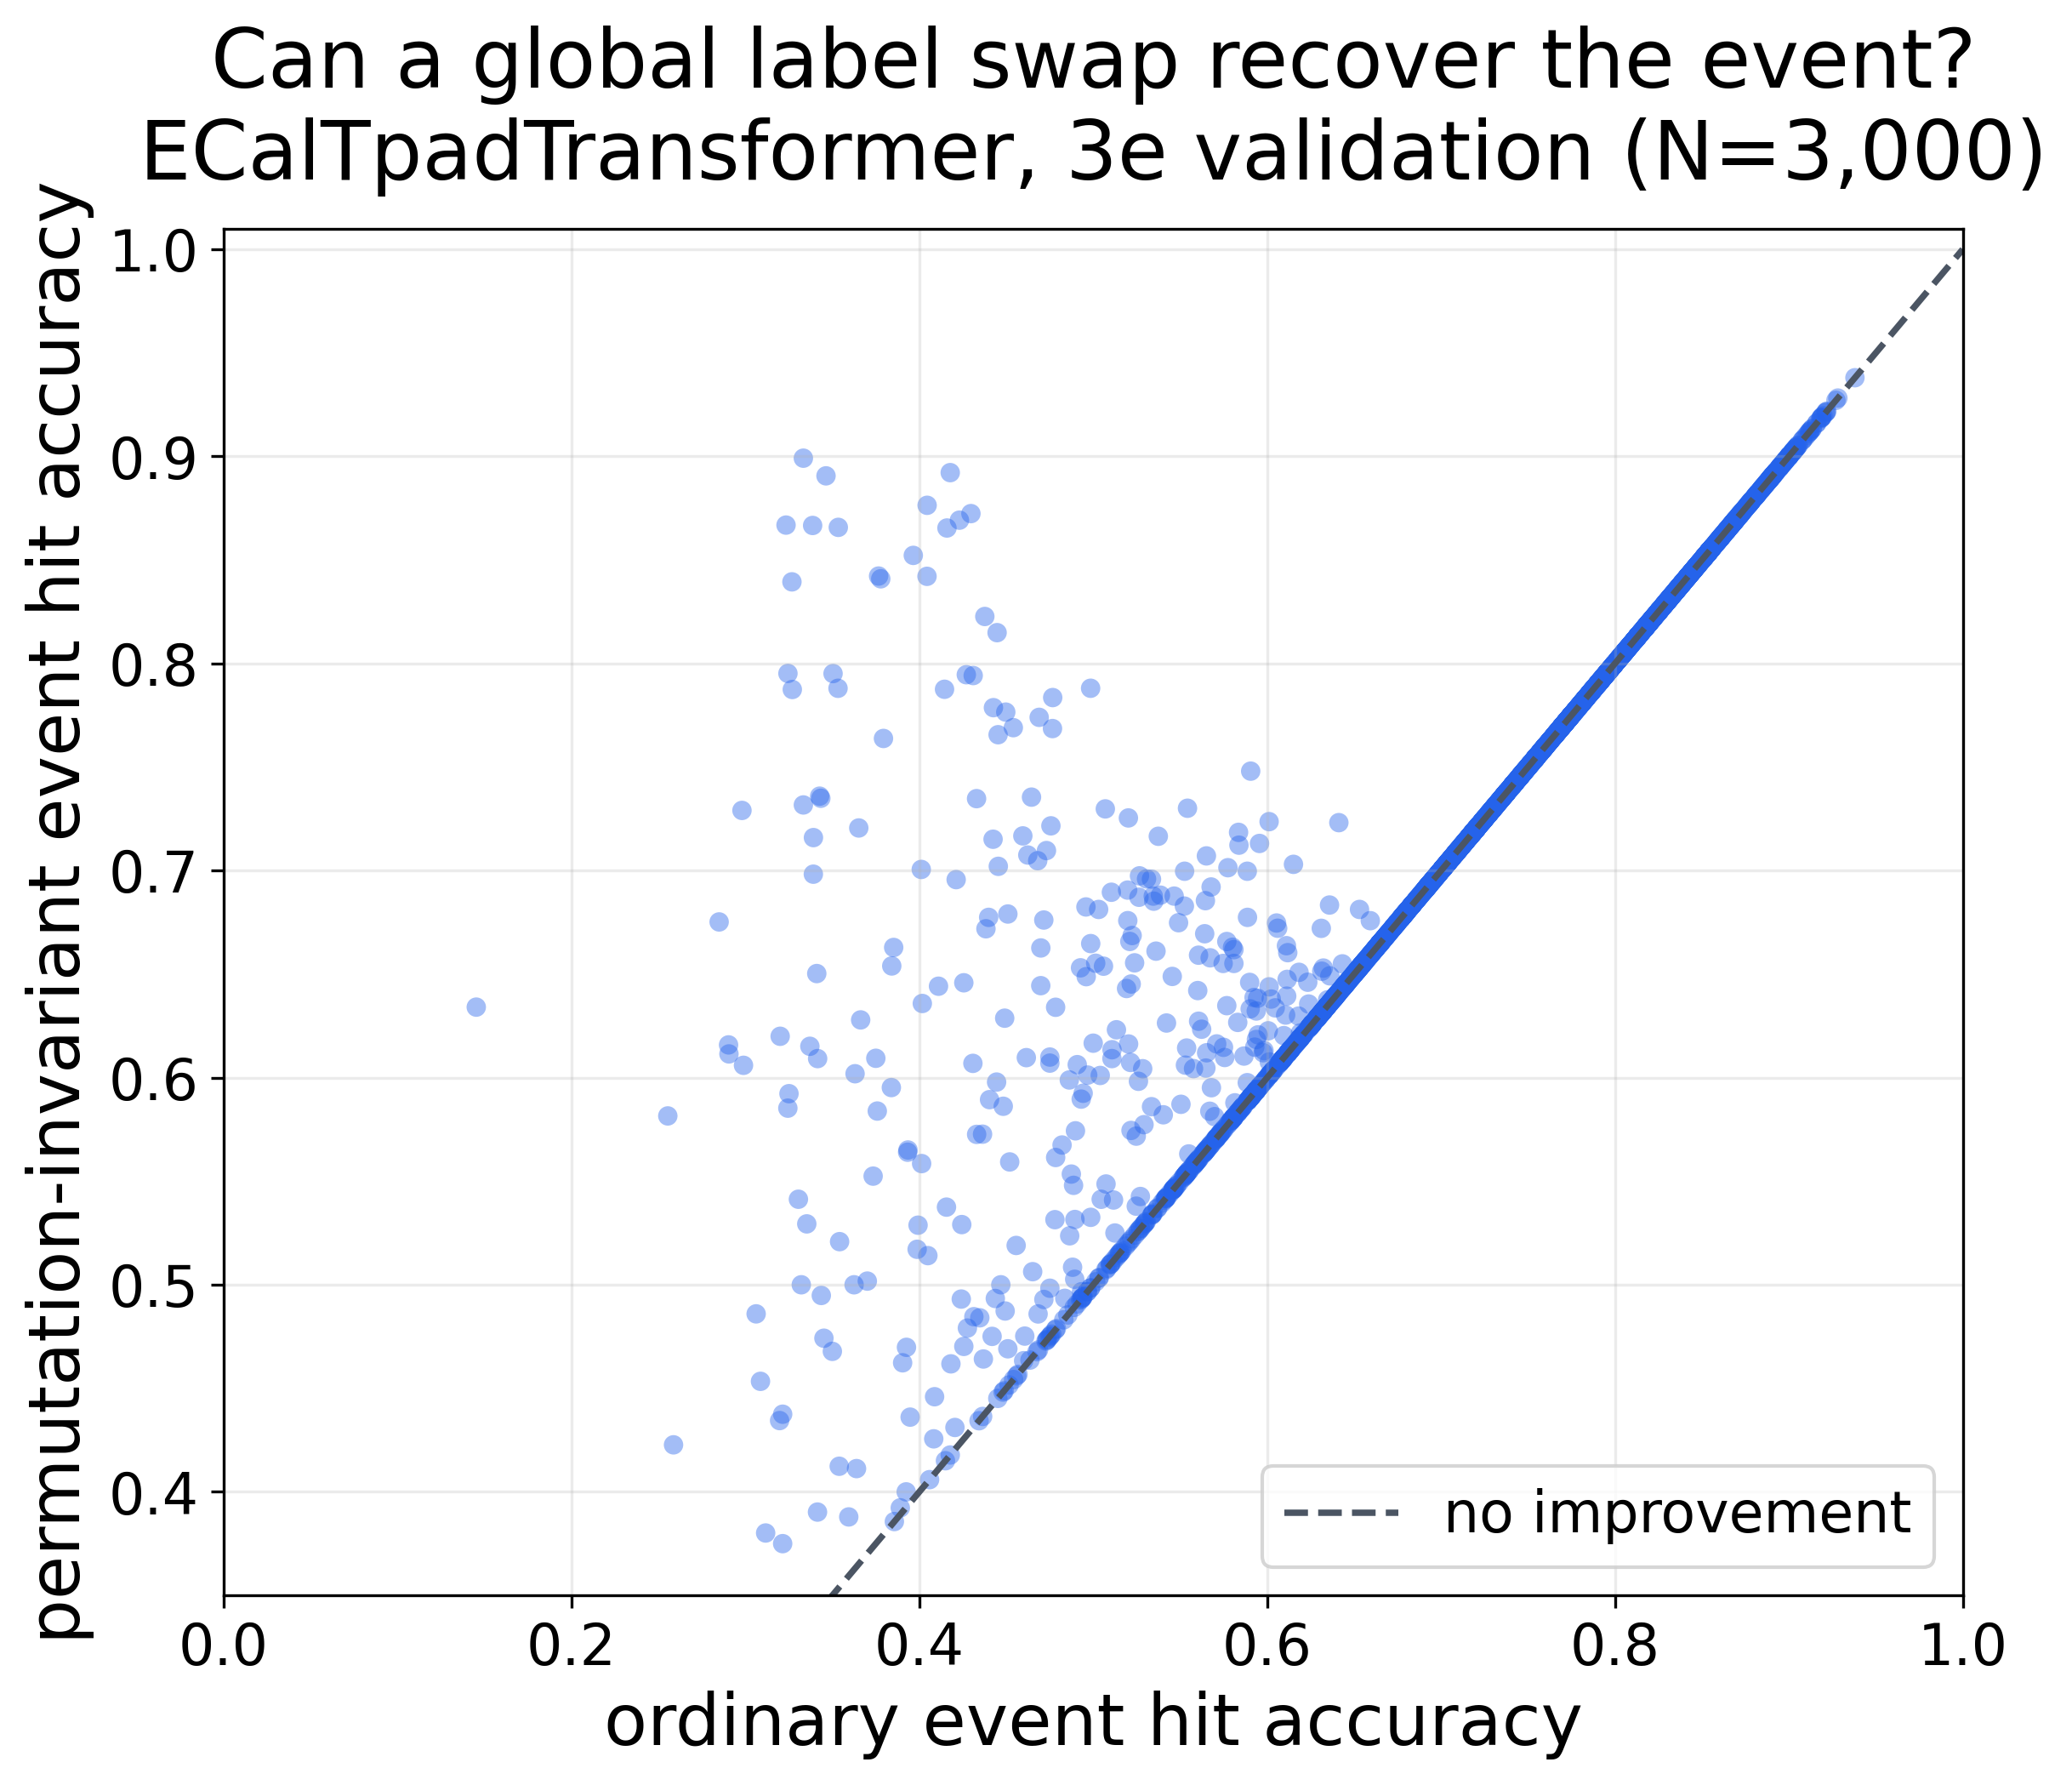
\includegraphics[width=\linewidth]{config/fig/results/shower_label_swap_recovery_3e.png}
    \caption{Canonical-label and permutation-aligned accuracy for \(3{,}000\)
    \(3e\) validation events. Alignment changes \(297\) scores
    (\(9.9\,\%\)) and increases the mean from \(0.722\) to \(0.737\).}
    \label{fig:results_label_swap_recovery}
    \vspace{-0.5\baselineskip}
\end{wrapfigure}

where \(N_{\mathrm{correct}}\) is the number of hits whose predicted label
matches the target label. Accuracy is calculated separately for every event
to show the distribution from easy to difficult events. A pooled accuracy is
also reported after combining the hits from all events; this gives events
with more hits greater weight.


The electron labels require one additional consideration. Their canonical
ordering is useful during training, but the numerical names of the predicted
shower groups are not themselves physical. A model can separate the hits into
the correct showers while exchanging two complete labels. To distinguish
such an exchange from incorrect grouping, every possible \emph{global} label
mapping is tested for each event: two mappings for a \(2e\) event and six for
a \(3e\) event. The mapping giving the highest ordinary hit accuracy is
retained. Equivalently,
\begin{equation}
    A_{\mathrm{perm}}
    =
    \max_{\pi} A_{\mathrm{hit}}(\pi),
    \label{eq:event_permutation_accuracy}
\end{equation}
where \(\pi\) denotes one global relabelling of the predicted groups. The same
mapping must be used for every hit in the event, so this cannot correct
individual classification errors. Unless stated otherwise, the reported
hit-assignment accuracies use this permutation-invariant alignment. Training
curves remain unaligned because training is performed against the canonical
targets.

Figure~\ref{fig:results_label_swap_recovery} shows the practical effect of the
alignment. Most event scores are unchanged, while a minority improve because
one global exchange better matches the truth labels.

A second accuracy gives more importance to hits carrying more reconstructed
energy. After applying the same event-level label mapping as above, it is
\begin{equation}
    A_E
    =
    \frac{\sum_{\text{correct hits}} E_h}
         {\sum_{\text{all hits}} E_h},
    \label{eq:event_energy_weighted_accuracy}
\end{equation}
where \(E_h\) is the untransformed reconstructed ECal energy. Thus,
\(A_E=1\) means that all reconstructed energy is carried by correctly assigned
hits. Comparing \(A_E\) with the unweighted accuracy indicates whether errors
preferentially occur on low- or high-energy hits. Pooled confusion matrices
are used separately to show which origin groups are confused.

\subsubsection{Prediction Confidence}

The model converts its output scores into normalised class scores (logits) with a
softmax function. The largest score is called the hit confidence. Normalised
entropy for hit \(h\) is
\begin{equation}
    H_h
    =
    -\frac{1}{\log K}
    \sum_{j=1}^{K} p_{hj}\log p_{hj},
    \label{eq:normalised_prediction_entropy}
\end{equation}
where \(p_{hj}\) is the softmax score for electron class \(j\) and \(K\) is
the number of classes. Dividing by \(\log K\), the largest possible entropy,
places \(H_h\) between zero and one. It is zero when one class receives all
weight and one when all classes are equally likely. Mean confidence and
entropy are calculated for each event and used as supporting diagnostics of
uncertainty and difficult events; neither changes the predicted hit label.


\subsubsection{Projected Shower Geometry}

To relate performance to physical overlap, every ECal hit is projected onto
the transverse \(x\)--\(y\) plane. For readability, the event index is omitted
below. Hit \(h\), with transverse position \(\boldsymbol r_h\), contributes
the following energy to truth shower \(j\):
\begin{equation}
    w_{hj}=E_h f_{hj},
    \label{eq:shower_geometry_weight}
\end{equation}
where \(E_h\) is the untransformed reconstructed hit energy and \(f_{hj}\) is
the simulated fraction deposited by electron \(j\). Consequently, a mixed hit
contributes to several truth showers in proportion to their deposited energy.

The centroid \(\boldsymbol\mu_j\) is the energy-weighted centre of shower
\(j\), and \(s_j\) is its root-mean-square transverse width:
\begin{align}
    \boldsymbol{\mu}_j
    &=
    \frac{\sum_h w_{hj}\boldsymbol r_h}
         {\sum_h w_{hj}},
    \label{eq:projected_shower_centroid} \\
    s_j
    &=
    \sqrt{
    \frac{\sum_h w_{hj}
    \lVert\boldsymbol r_h-\boldsymbol\mu_j\rVert_2^2}
         {\sum_h w_{hj}}},
    \label{eq:projected_shower_width}
\end{align}
For two showers \(i\) and \(j\), their centroid distance \(d_{ij}\) is divided
by their combined width to obtain the dimensionless separation \(S_{ij}\):
\begin{align}
    d_{ij}
    &=
    \lVert\boldsymbol\mu_i-\boldsymbol\mu_j\rVert_2,
    \label{eq:shower_centroid_distance} \\
    S_{ij}
    &=
    \frac{d_{ij}}{\sqrt{s_i^{2}+s_j^{2}}}.
    \label{eq:normalised_shower_separation}
\end{align}
For an event with several electrons, the smallest pairwise value is used:
\begin{equation}
     S_{\min}=\min_{i<j}S_{ij}.
    \label{eq:min_shower_separation}
\end{equation}
A small \(S_{\min}\) means that at least two showers are close compared with
their widths and are therefore strongly overlapping. Geometry is evaluated
either over all ECal layers or over an explicitly stated early-layer subset.
Because the weights use simulated energy fractions, this is a truth-assisted
difficulty measure rather than an observable available on detector data.

\subsubsection{Difficulty Profiles and Multi-Task Metrics}

Accuracy profiles use approximately equal-population bins in shower
separation or model confidence. Means and \(95\,\%\) confidence intervals are
estimated by bootstrap resampling events within each bin. Events are also
ranked by permutation-aligned hit accuracy to select lower-tail, median and
high-performing examples.

For the multi-task model, the predicted energy fractions are evaluated with
the mean absolute error (MAE):
\begin{equation}
    \operatorname{MAE}_{f}
    =
    \operatorname{mean}_{h,j}
    \left|\widehat f_{hj}-f_{hj}\right|,
    \label{eq:fraction_mae}
\end{equation}
where \(f_{hj}\) and \(\widehat f_{hj}\) are the true and predicted fractions
for hit \(h\) and output slot \(j\). The mean covers every retained ECal hit
and the four fraction components: background and the three possible electron
slots. An MAE of zero is perfect; an MAE of \(0.10\) means that a predicted
fraction differs from its target by \(0.10\), or ten percentage points, on
average. The metric is reported both before and after invalid electron slots
are masked during post-processing.

The remaining multi-task metrics have direct counting interpretations. Exact
contributor-set accuracy requires the complete predicted set of contributing
electrons to match the truth set. Dominant-origin accuracy considers only the
electron with the largest predicted fraction. Mixed-hit precision is the
fraction of predicted mixed hits that are truly mixed, while recall is the
fraction of truly mixed hits that the model identifies. Electron-count
accuracy is the fraction of events with the correct number of valid electron
slots.

Selected events are inspected with Plotly-based interactive HTML displays that
preserve the detector \(z\)-coordinate. A menu switches among truth,
prediction, correctness, confidence, entropy and energy, while hover labels
expose hit-level values. These displays support qualitative checks and
failure-mode discovery; an example is shown in
Figure~\ref{fig:interactive_event_display} in the Appendix.~\ref{sec:appendix_diagnostics}.
